% chapters/12/section-02.tex
\section{Antarmuka Unity}
\label{sec:antarmuka-unity}

Ketika sebuah \istilah{project} dibuka untuk pertama kalinya, yang tampak
adalah beberapa panel yang saling berdampingan. Bagian ini menjelaskan kegunaan
masing-masing, sesuai indikator \ind{a}.

\subsection{Empat Panel Utama}

Antarmuka Unity tersusun atas empat panel yang paling sering dipakai. Susunan
bawanya diperlihatkan pada Gambar~\ref{fig:editor-unity}.

\begin{figure}[htbp]
\centering
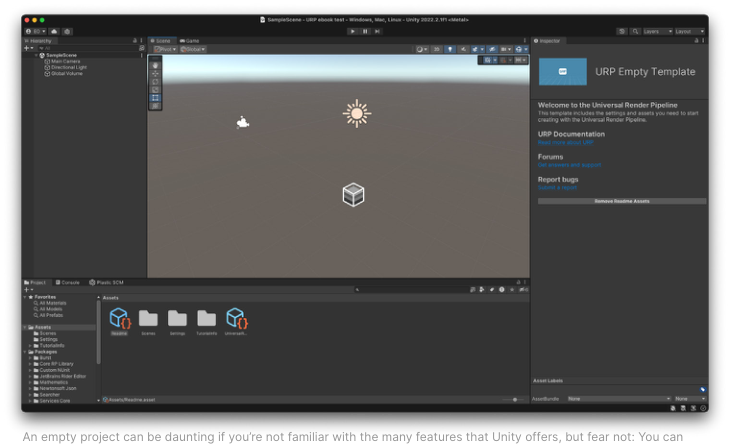
\includegraphics[width=0.94\textwidth]{figures/editor-unity.png}
\caption{Antarmuka Unity dengan empat panel utama pada susunan bawaannya}
\label{fig:editor-unity}
\sumber{[R12] halaman 42, dengan penyesuaian keterangan}
\end{figure}

\begin{description}
  \item[\istilah{Hierarchy}] Terletak di kiri atas. Memuat daftar seluruh benda
        yang berada pada \istilah{scene} yang sedang dibuka, beserta hubungan
        kekeluargaannya. Panel ini menjawab pertanyaan ``benda apa saja yang ada
        di sini?''.
  \item[\istilah{Scene}] Terletak di tengah, dan merupakan panel terluas.
        Menampilkan scene dari sudut pandang perancang, sehingga benda dapat
        dipindahkan dan diatur dengan menunjuknya langsung. Panel ini menjawab
        pertanyaan ``bagaimana susunan ruangnya?''.
  \item[\istilah{Inspector}] Terletak di kanan. Menampilkan seluruh komponen
        benda yang sedang dipilih, beserta nilai setiap pengaturannya. Panel ini
        menjawab pertanyaan ``benda ini tersusun atas apa, dan bagaimana
        pengaturannya?''.
  \item[\istilah{Project window}] Terletak di bawah. Memuat seluruh berkas
        \istilah{project}, yaitu scene, \istilah{script}, gambar, bunyi, dan
        aset lainnya. Panel ini menjawab pertanyaan ``berkas apa saja yang
        dimiliki project ini?''.
\end{description}

Perhatikan perbedaan antara \istilah{Hierarchy} dan \istilah{Project window},
sebab keduanya sama-sama berupa daftar. \istilah{Hierarchy} memuat benda yang
ada \textbf{di dalam scene yang sedang dibuka}, sedangkan
\istilah{Project window} memuat \textbf{seluruh berkas} yang dimiliki project,
termasuk scene lain yang belum dibuka. Sebuah berkas scene tidak tampak pada
\istilah{Hierarchy}, dan sebuah benda di dalam scene tidak tampak pada
\istilah{Project window}.

\subsection{Panel Lain yang Perlu Diketahui}

Dua panel lain akan sering Anda pakai pada bab-bab berikutnya.

\begin{itemize}
  \item \istilah{Game} menampilkan scene dari sudut pandang kamera permainan,
        yaitu apa yang akan dilihat pemain. Panel ini dipakai untuk memeriksa
        hasil pekerjaan Anda.
  \item \istilah{Console} menampilkan pesan yang ditulis kode Anda melalui
        \code{Debug.Log}, beserta peringatan dan kesalahan. Panel ini
        menggantikan terminal pada blok Python.
\end{itemize}

\begin{tipsbox}
Kebiasaan yang menghemat waktu: biasakan memastikan panel mana yang sedang
aktif sebelum menekan tombol. Sebagian besar tombol pintas Unity bergantung
pada panel yang sedang aktif, sehingga penekanan yang sama dapat berarti
berbeda. Apabila sebuah tombol pintas tidak bekerja seperti dugaan, periksa
lebih dahulu panel mana yang sedang aktif.
\end{tipsbox}

\begin{catatabox}
Susunan panel dapat diubah dengan menggeser judulnya, dan susunan itu disimpan
di dalam \istilah{project}. Apabila Anda menemukan susunan yang lebih nyaman,
simpanlah sebagai susunan baru melalui menu \istilah{Layout} pada sudut kanan
atas. Untuk keperluan pembelajaran, susunan bawaan sudah memadai.
\end{catatabox}
